\section{Messergebnisse und Auswertung}

\subsection{Teil I: Pockels-Effekt}

\subsubsection{Sägezahnmethode}

\begin{figure}[H]
\begin{center}
  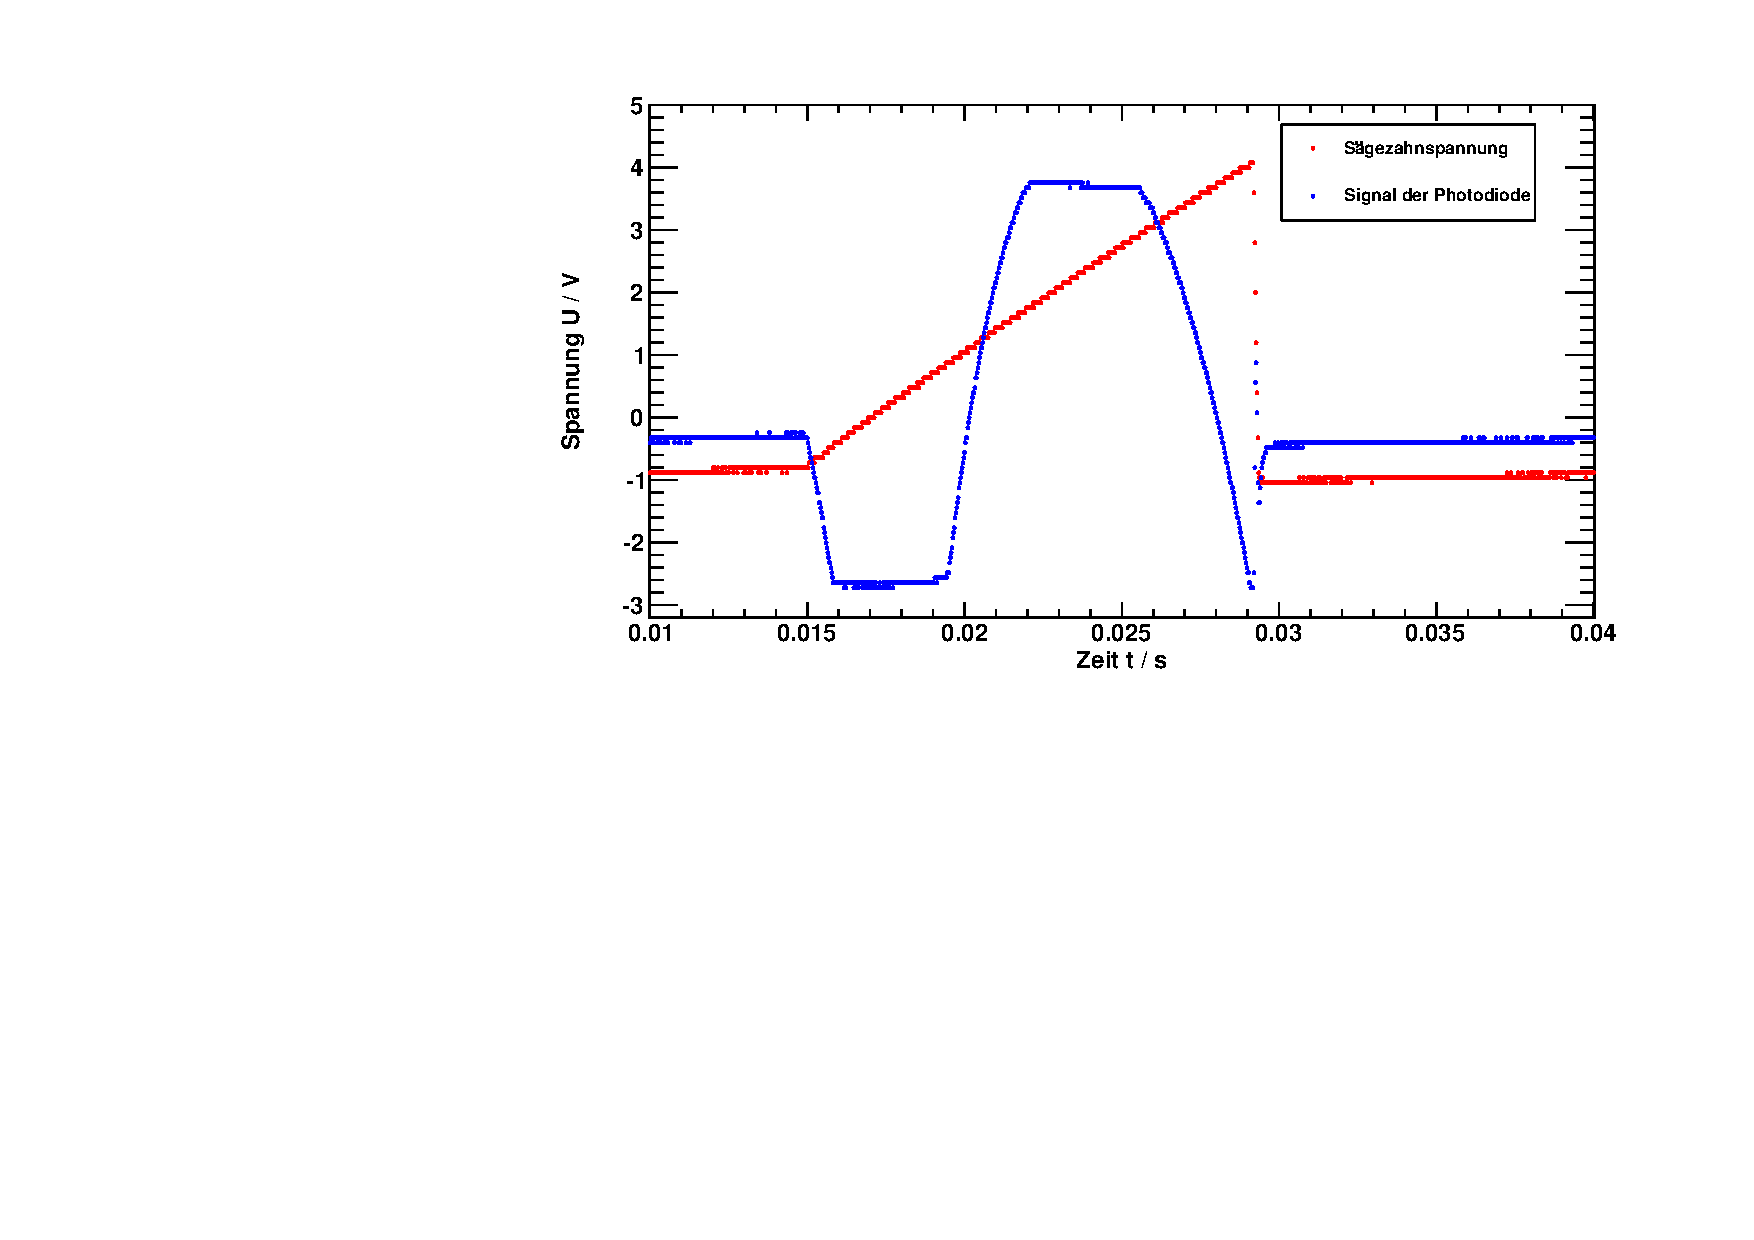
\includegraphics[width=15cm]{../img/pock_saege_winkel0.pdf}
  \caption{Deformiertes Photodiodensignal (blau) bei Einstellung der Polarisationsachse des Analysators in
  Richtung höchster Transmission der Pockelszelle.}
  \label{img:pock_saege_winkel0}
\end{center}
\end{figure}

\autoref{img:pock_saege_winkel0} zeigt das Photodiodensignal, wenn der Analysator so eingestellt wird,
wie in der Versuchsanleitung beschrieben, so dass die Amplitude des Photodiodensignals maximiert wird.
Diese Einstellung ist zum Ablesen von Maximum und Minimum des Signals nicht geeignet.
\autoref{img:pock_saege_winkel1}, \autoref{img:pock_saege_winkel2} und \autoref{img:pock_saege_winkel3}
zeigen Messungen mit niedrigerer Amplitude, die für die Auswertung verwendet wurden.

\begin{figure}[H]
\begin{center}
  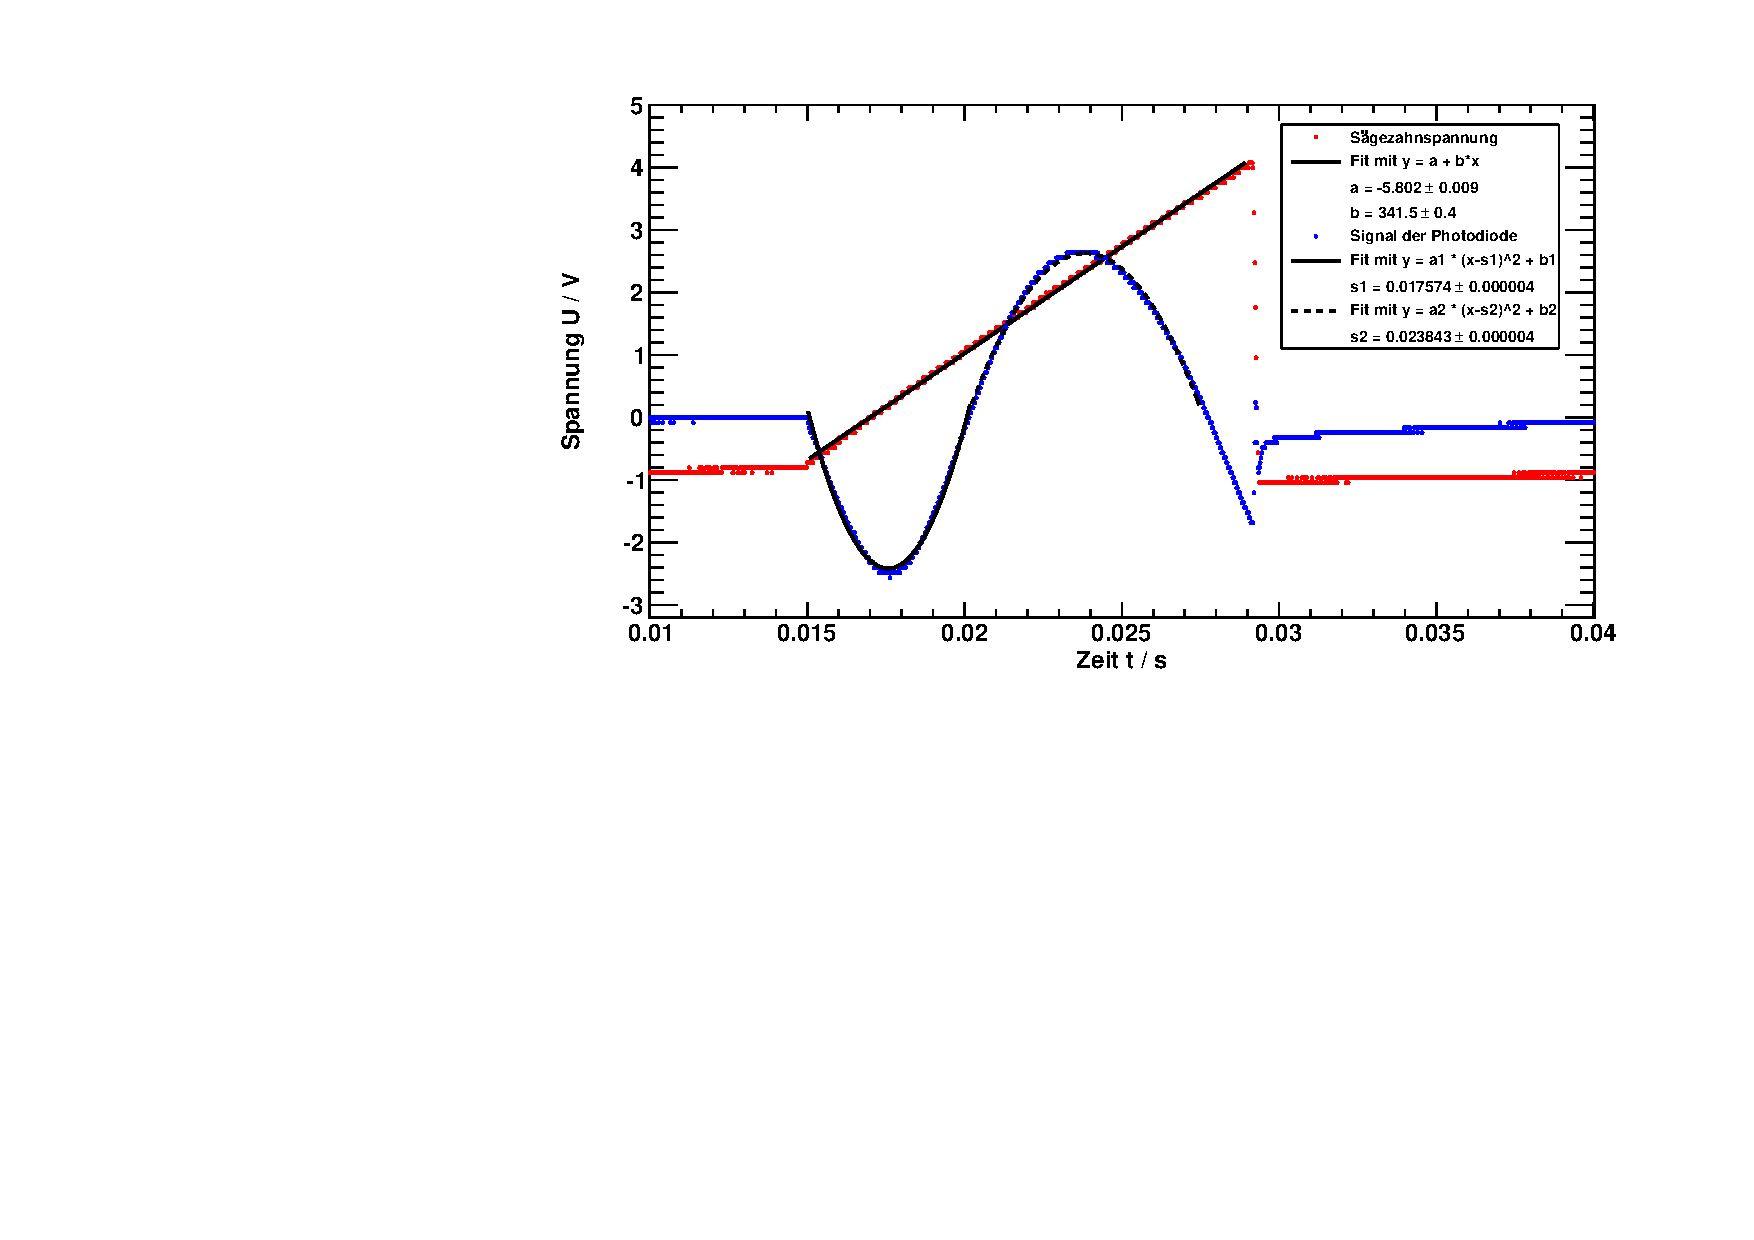
\includegraphics[width=15cm]{../img/pock_saege_winkel1.pdf}
  \caption{capt.}
  \label{img:pock_saege_winkel1}
\end{center}
\end{figure}

\begin{figure}[H]
\begin{center}
  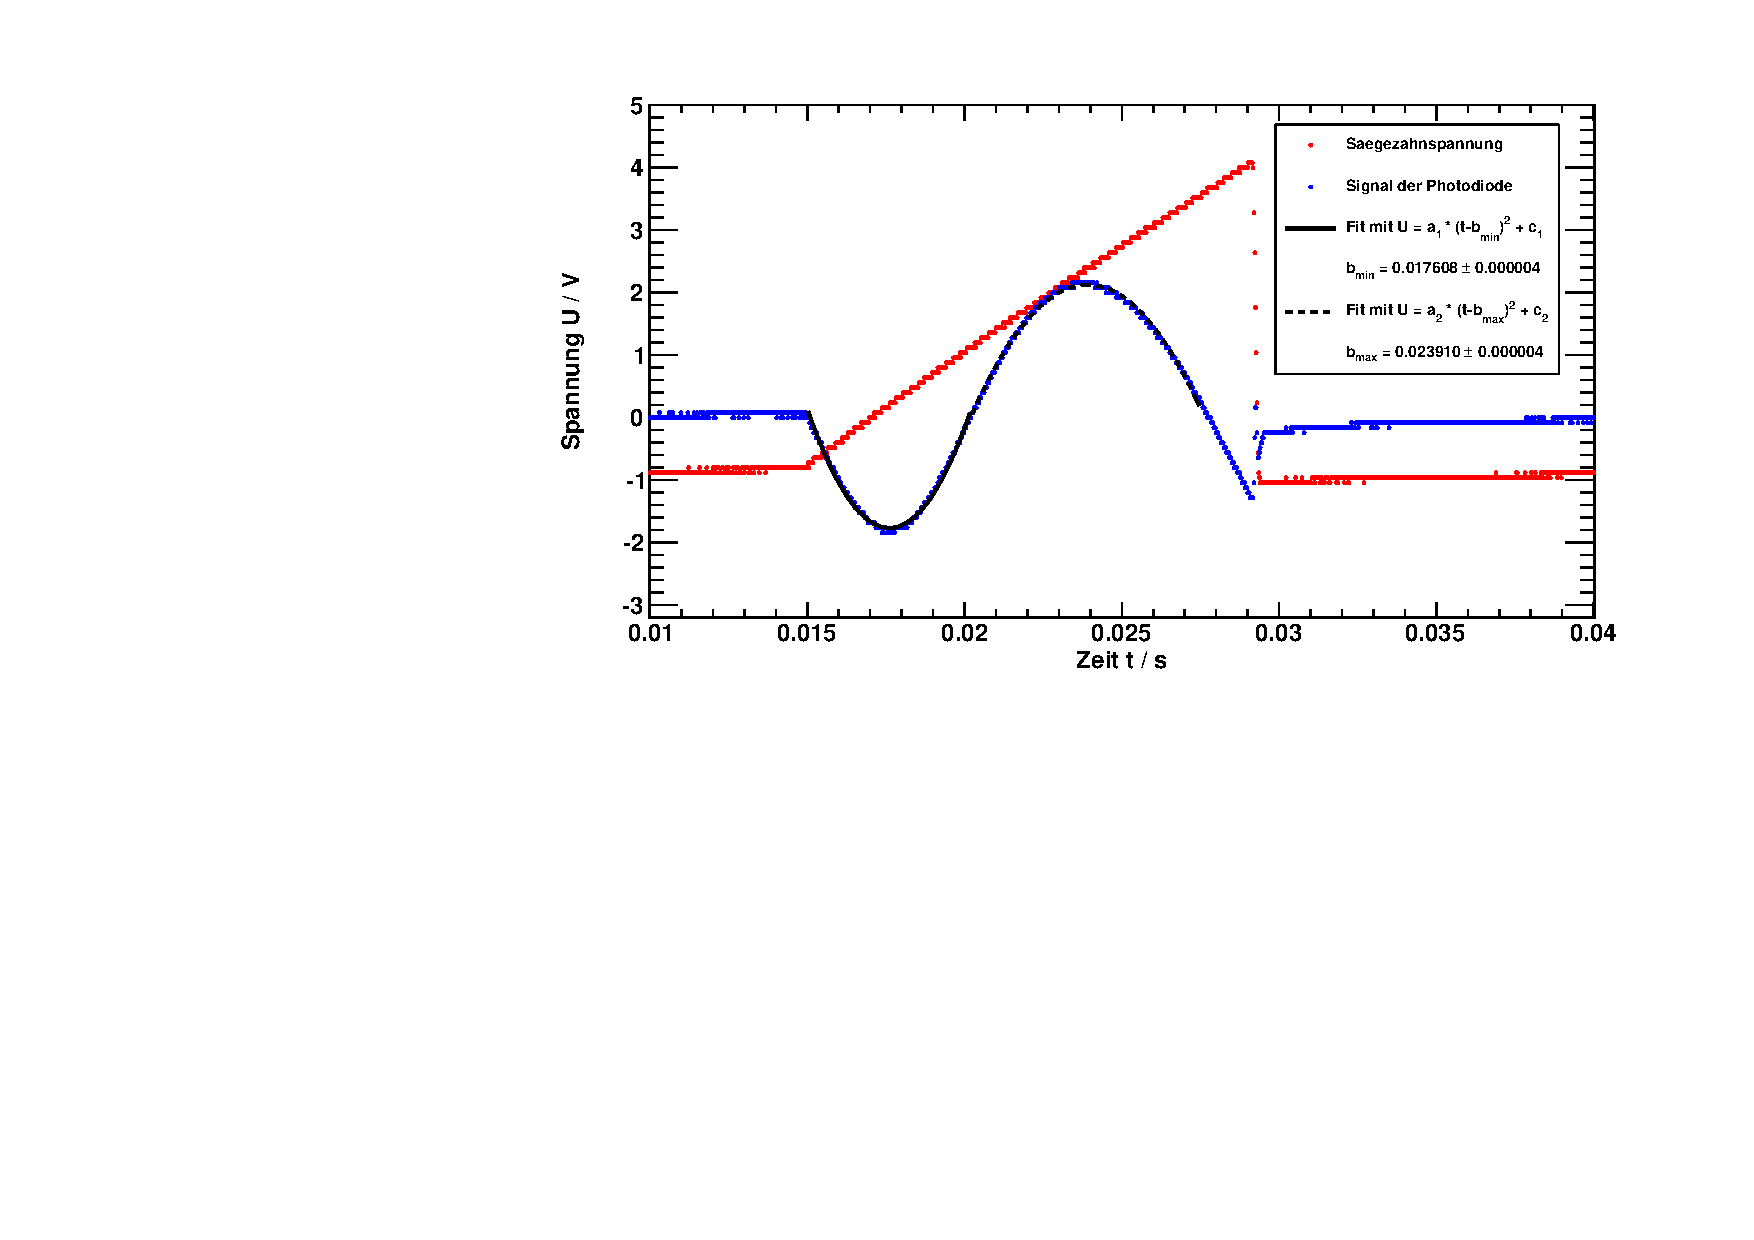
\includegraphics[width=15cm]{../img/pock_saege_winkel2.pdf}
  \caption{capt.}
  \label{img:pock_saege_winkel2}
\end{center}
\end{figure}

\begin{figure}[H]
\begin{center}
  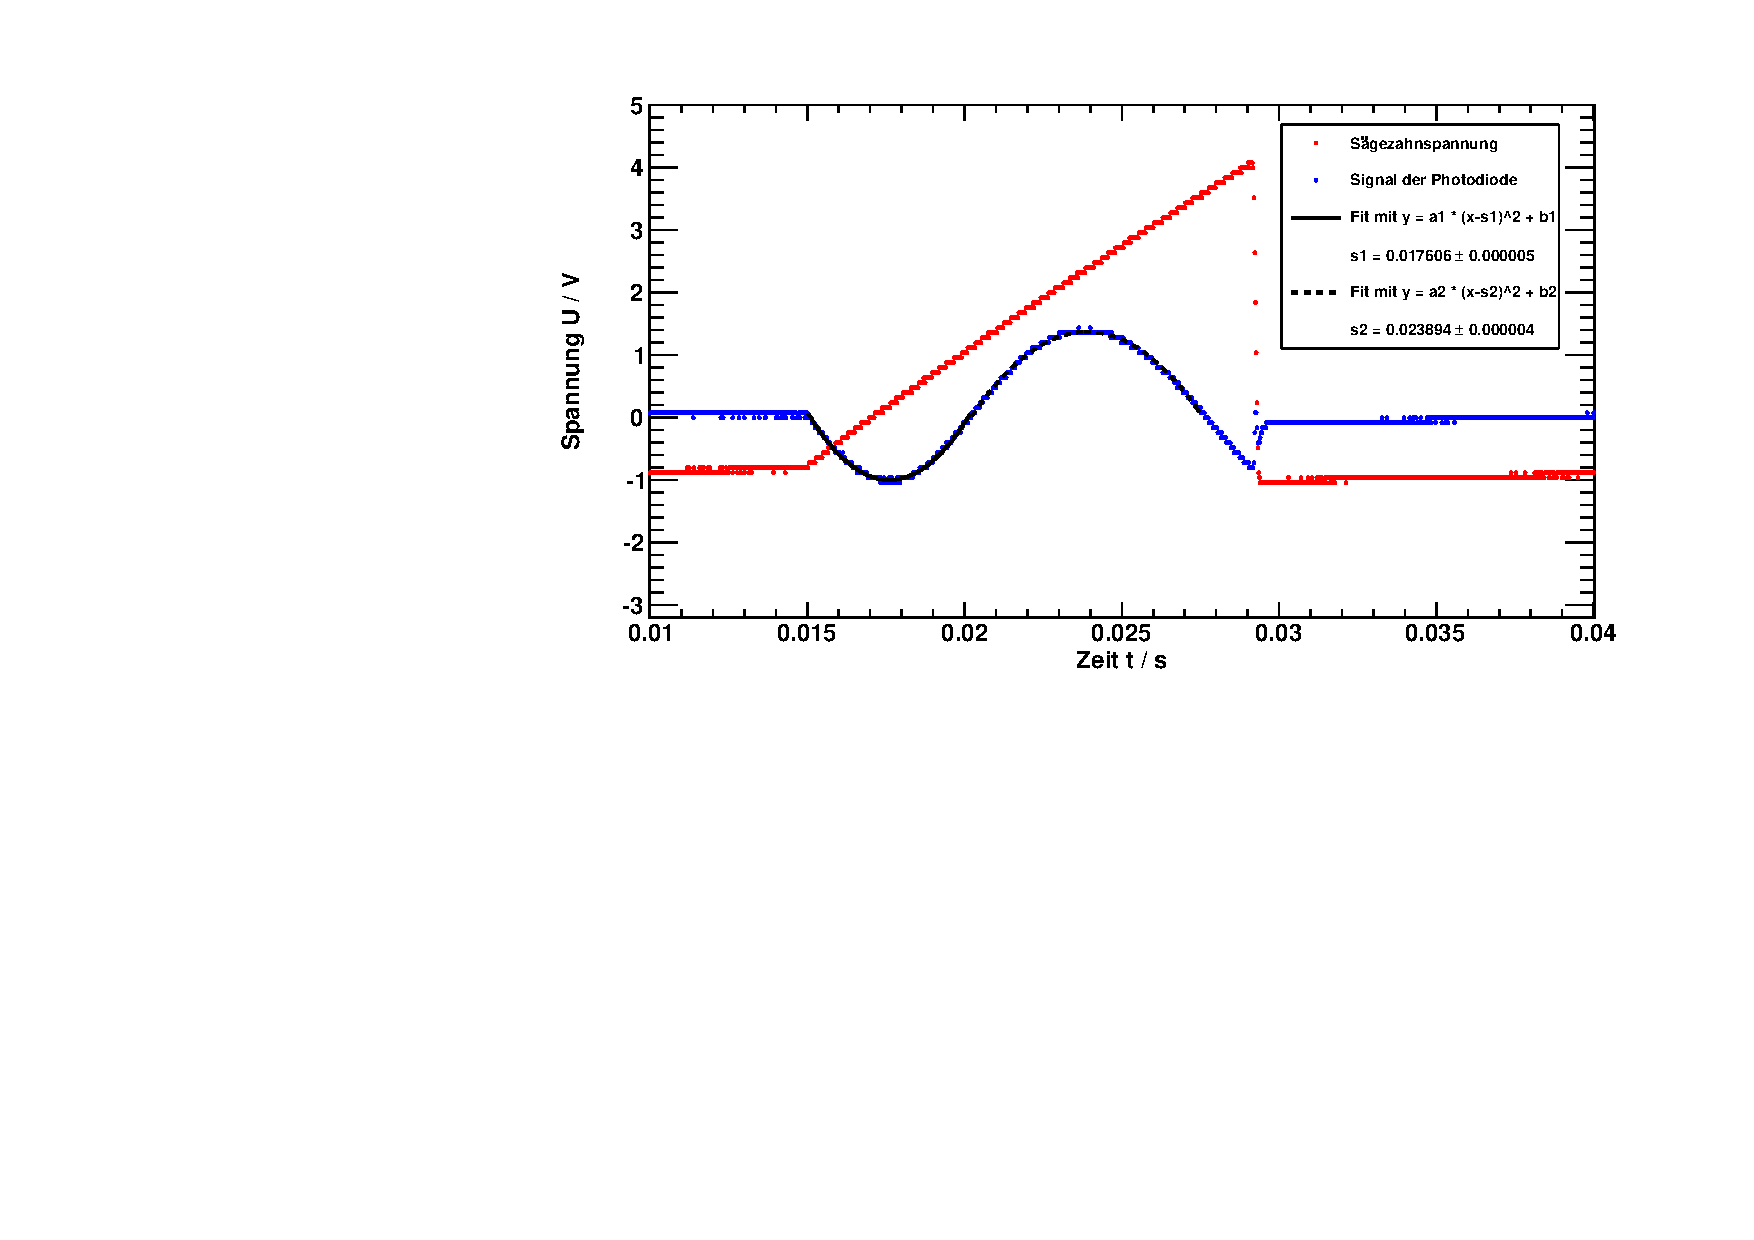
\includegraphics[width=15cm]{../img/pock_saege_winkel3.pdf}
  \caption{capt.}
  \label{img:pock_saege_winkel3}
\end{center}
\end{figure}

In \autoref{tab:minmax} sind die Positionen von Maximum und Minimum für die drei Messungen aufgeführt.
Diese Positionen wurden durch Fits von Parabeln (mit den Fitparametern $a$, $b$ und $c$) an die Messdaten gewonnen:
\begin{equation}
  y = a \cdot (x-b)^2 + c
\end{equation}
Minimum und Maximum wurden hier mit separaten Parabeln gefittet,
weil das Signal offensichtlich kein Sinus ist und ein sinusförmiger Fit keine gute Beschreibung liefert.
Der Parameter $b$ ist die Position des Extremums auf der x-Achse, die für die weitere Auswertung relevant ist.\\
Aus der Position des Maximums $b_{\text{max}}$ und der des Minimums $b_{\text{min}}$
wurde die Differenz $\Delta b$ gebildet:
\begin{equation}
  \Delta b = b_{\text{max}} - b_{\text{min}} \ , \qquad s_{\Delta b} = \sqrt{s_{b_{\text{max}}}^2 + s_{b_{\text{min}}}^2}
\end{equation}
Auch die drei Werte für $\Delta b$ sind in \autoref{tab:minmax} aufgeführt.
\begin{table}[H]
\caption{Position von Maximum und Minimum auf der x-Achse und Positionsdifferenz für die
drei Messungen.}
\begin{center}
\begin{tabular}{|c|c|c|c|c|c|c|}
  \hline
 Messung		& $b_{\text{min}}$ / s 	& $s_{b_{\text{min}}}$ / s 	& $b_{\text{max}}$ / s 	& $s_{b_{\text{max}}}$ / s 	& $\Delta b$ / s 	& $s_{\Delta b}$ / s \\ \hline  
 1 				& 0.017574      		& 0.000004     				& 0.023843   			& 0.000004        			& 0.006269   		& 0.000006       \\ \hline  
 2   		  	& 0.017608       		& 0.000004     				& 0.023910     			& 0.000004        			& 0.006302      	& 0.000005       \\ \hline  
 3 	    		& 0.017606       		& 0.000005     				& 0.023894    			& 0.000004       			& 0.006288    		& 0.000006      \\ \hline   
 
\end{tabular}
\end{center}
\label{tab:minmax}
\end{table}
Im Experiment wurde die Amplitudenabhängigkeit der Messwerte untersucht.
Es ist kein signifikanter Trend erkennbar; die Werte für $\Delta b$ stimmen im 3-\textsigma -Intervall
überein.
Deshalb erscheint es gerechtfertigt,
den gewichteten Mittelwert $\overline{\Delta b}$ aus den drei Werten zu bilden. Man erhält
\begin{equation}
  \overline{\Delta b} = (0.006287 \pm 0.000003)\,\text{s}
\end{equation}




Die Steigung der Sägezahnfunktion wird mit einem Steigungsdreieck abgeschätzt,
die Positionen der Ecken des Dreiecks befinden sich in \autoref{tab:steigungsdreieck}.
\begin{table}[H]
\caption{Messwerte zur Berechnung der Steigung der Sägezahnfunktion.}
\begin{center}
\begin{tabular}{|c|c|c|c|c|}
  \hline
   				& $U$ / V 	& $s_U$ / V & $t$ / s 	& $s_t$ / s \\ \hline  
 Einsatzpunkt 	& -0.8      & 0.1     	& 0.0149   	& 0.0002       \\ \hline  
 Maximum     	& 4.1      	& 0.1     	& 0.0291    & 0.0002       \\ \hline   
 
\end{tabular}
\end{center}
\label{tab:steigungsdreieck}
\end{table}
Man erhält mit den Messwerten für die Steigung der Sägezahnfunktion $m_s$:
\begin{equation}
  m_s = \frac{U_M-U_E}{t_M-t_E} = 50 \,\frac{\text{V}}{\text{s}}
\end{equation}
Für den Fehler darauf folgt mit dem Gaußschen Fehlerfortpflanzungsgesetz
\begin{equation}
  s_{m_s}=1
\end{equation}





\subsubsection{Modulierte Gleichspannung}

\subsection{Teil II: Faraday-Effekt}
\subsubsection{Bestimmung der Verdet-Konstante}
Für jede Spannung wurde vier mal ($N=4$) der entsprechende Winkel gemessen. Der Fehler einer Einzelmessung des Winkels wurde auf
\begin{equation}
  s_{\alpha_i} = 0.2^\circ
\end{equation}  % TODO Fehler auf Strom
geschätzt. Es wird zunächst der Mittelwert der Winkel gebildet:
\begin{equation}
  \alpha = \sum_{i=1}^{N} \alpha_i, \qquad s_{\alpha} = \frac{s_{\alpha_i}}{\sqrt{N}}
\end{equation}
Die Spannungen und gemittelten Winkel werden nun mit einer Geraden gefittet:
\begin{equation}
  \alpha(I) = a + b \cdot I
\end{equation}
Die Werte und der Fit sind in \autoref{img:faraday} dargestellt. Der Fit ergab folgende Werte:
\begin{equation}
\begin{split}
  \label{eq:faraday:params}
  a &= (-0.28 \pm 0.06)\,{}^\circ \\
  b &= (2.5769 \pm 0.0199)\,\frac{{}^\circ}{\text{A}}
\end{split}
\end{equation}
\begin{figure}[H]
\begin{center}
  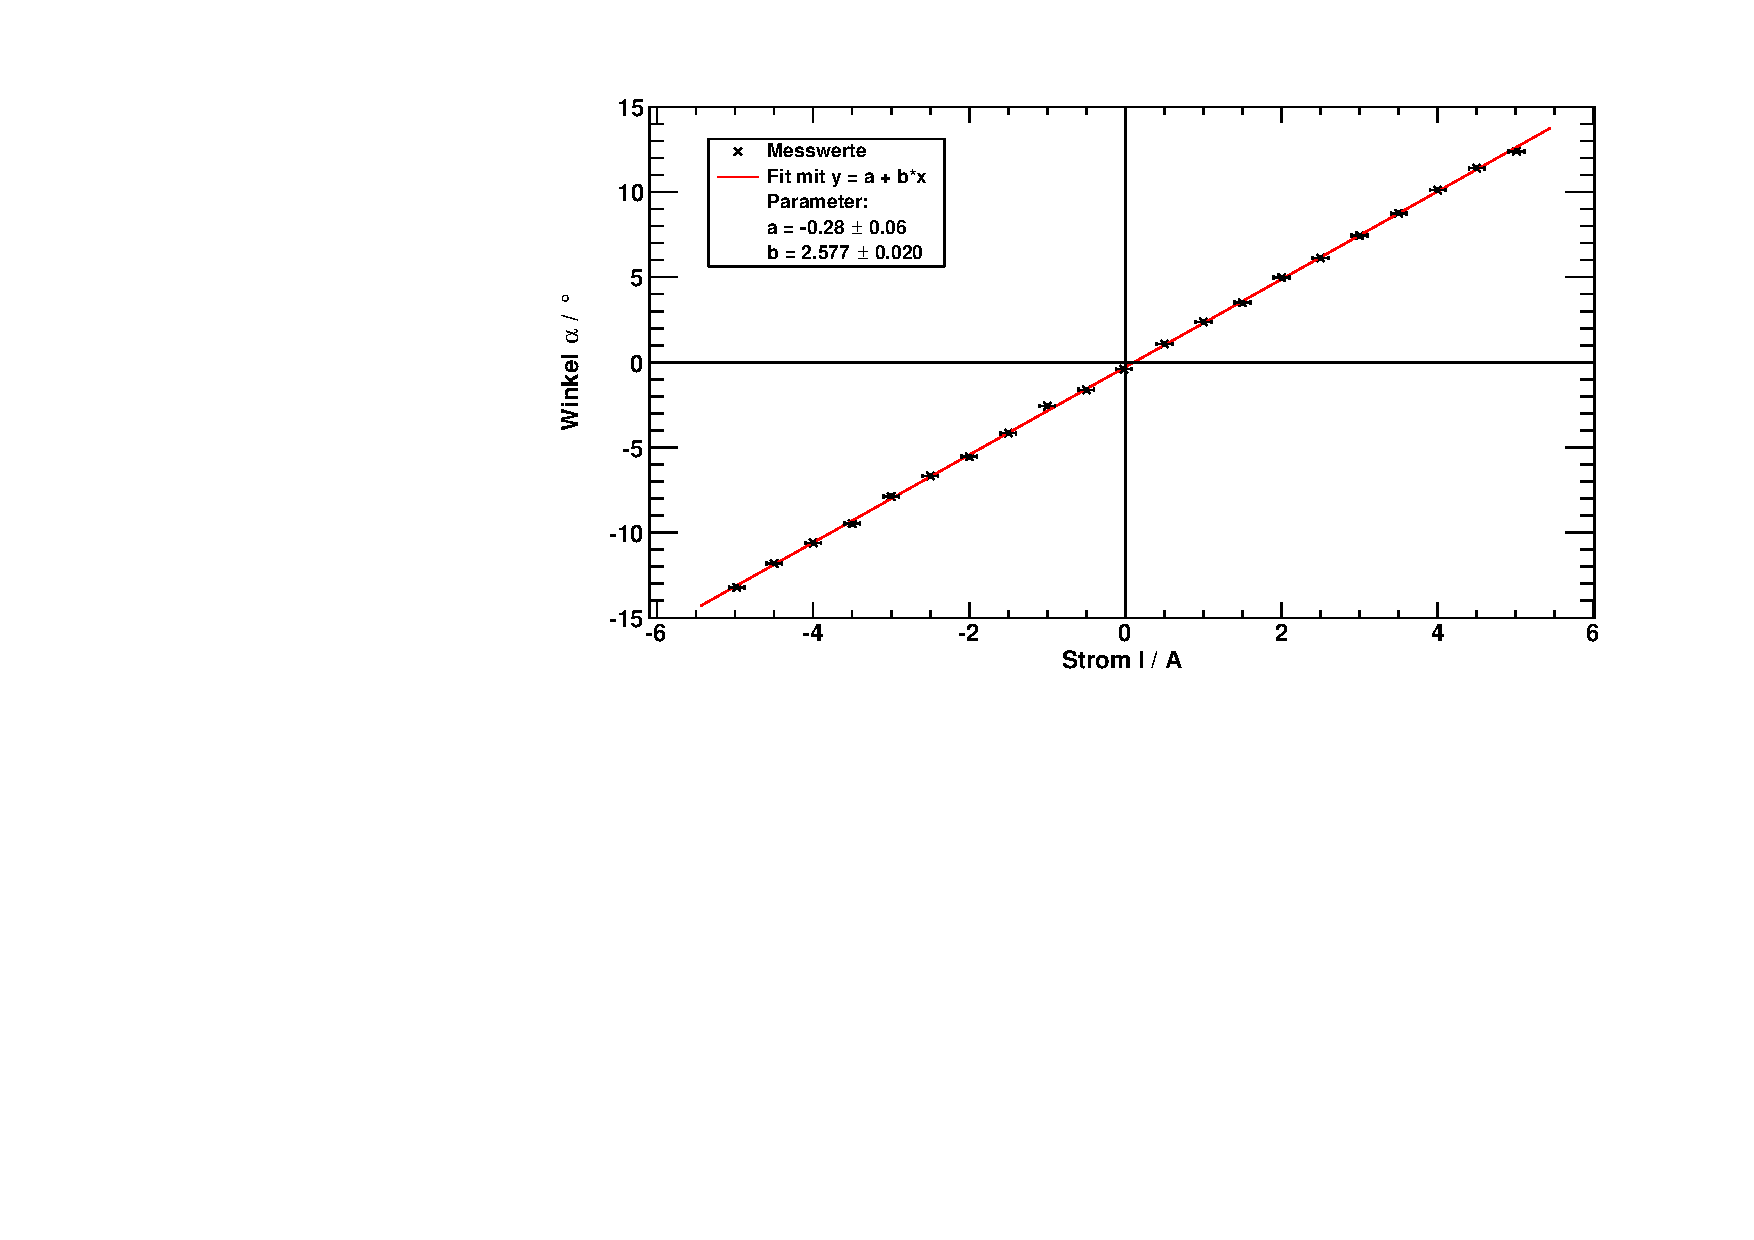
\includegraphics[width=\textwidth]{../img/faraday.pdf}
  \caption{Winkel $\alpha$ in Abhängigkeit des Stroms $I$ mit Fit einer Geraden.}
  \label{img:faraday}
\end{center}
\end{figure}
Mit \autoref{eq:verdet} wird nun die Verdet-Konstante $V$ berechnet:
\begin{equation}
  V = \frac{m}{2556}, \qquad s_V = \frac{s_m}{2556}
\end{equation}
\begin{equation}
  V = (1.008 \pm 0.008) \cdot 10^{-3}\,\frac{{}^\circ}{\text{A}}
\end{equation}
Die Verdet-Konstante rechnet man folgendermaßen in $\frac{\text{min}}{\text{Oe}\cdot \text{cm}}$ um:
\begin{equation}
  1\,\frac{{}^\circ}{\text{A}} = \frac{60\cdot 79.58}{100}\,\frac{\text{min}}{\text{Oe}\cdot \text{cm}}
\end{equation}
Es folgt für den berechneten Wert:
\begin{equation}
  V = (0.0481 \pm 0.0004)\,\frac{\text{min}}{\text{Oe}\cdot \text{cm}}
\end{equation}
Der Hersteller gibt:
\begin{equation}
  V^{\text{Herst.}} = 0.05\,\frac{\text{min}}{\text{Oe}\cdot \text{cm}}
\end{equation}
als Wert an. Der gemessene Wert stimmt innerhalb des $5-\sigma$-Intervalls mit 



\subsubsection{Bestimmung von $\epsilon$}
